\documentclass[10pt]{beamer}

\usetheme[progressbar=frametitle]{metropolis}
\usepackage{appendixnumberbeamer}
\usepackage{graphicx}
\usepackage{booktabs}
\usepackage[scale=2]{ccicons}
\usepackage[font=footnotesize,labelfont=bf]{caption}
\usepackage{mwe}

\usepackage{pgfplots}
\usepgfplotslibrary{dateplot}

\usepackage{xspace}
\newcommand{\themename}{\textbf{\textsc{metropolis}}\xspace}

\title{Icelandic Rock Ptarmigan Species Distribution Model}
\subtitle{}
% \date{\today}
\date{}
\author{Stefano Fochesatto}

\begin{document}

\maketitle


\begin{frame}{Icelandic Rock Ptarmigan Species Distribution Model}
    \begin{itemize}
        \item Using occurrence data to model Icelandic Rock Ptarmigan species distribution.
        \vfill
        \item These nationwide models are a first step for making science based decisions with respect to conservation management.
        \vfill
        \item Wildlife-livestock conflict and ecosystem degradation.  
    \end{itemize}
\end{frame}



\begin{frame}{The Data}
\begin{itemize}
    \item Study put together through several Icelandic environmental agencies, in conjunction with the University of Iceland and the UAF Institute of 
    Arctic Biology. 
    \vfill
    \item Nationwide and long term (1860-2021) Rock ptarmigan occurrence data (GBIF). 
    \vfill
    \item Separate occurrence data from the Icelandic Institute of Natural History (2005-2010) for model validation.
     \vfill
    \item 11 Environmental Layers (May, June, July of 2021).
\end{itemize}
\end{frame}


\begin{frame}{The Data}
    \begin{itemize}
        \item None of the environmental layers showed correlation above .75 (multicollinearity).
        \item Environmental layers consisted of:
        \begin{itemize}
            \item Three categorical variables: land cover classes, soil types, wilderness.
            \item Eight continuous variables: elevation, distance fenced pastures, distance to
            (inland) water, Normalized Difference Vegetation Index (NDVI), slope, and average
            precipitation, temperature and wind speed for June, July and August.
        \end{itemize}
    \end{itemize}
    \end{frame}
    






\begin{frame}{The Data}
   \begin{center}
    \begin{figure}
        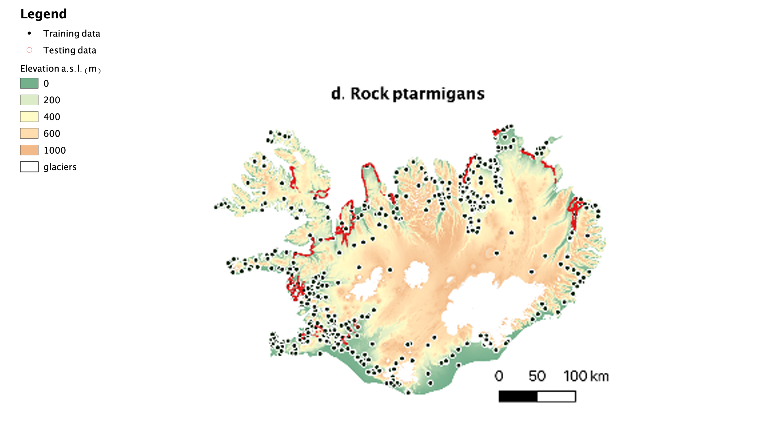
\includegraphics[width = \textwidth]{RockPtarmigan.png}
    \caption{Predicted distribution of herbivores in Iceland \dots Boulanger-Lapointe, Ágústsdóttir, et.al (in review)} 
\end{figure}
\end{center}
\end{frame}




\begin{frame}{Species Distribution Models}
    \begin{itemize}
        \item Using presence only data for SDM (specifically decision tree ensembles).
    \end{itemize}
    
    \begin{center}
        \begin{figure}
        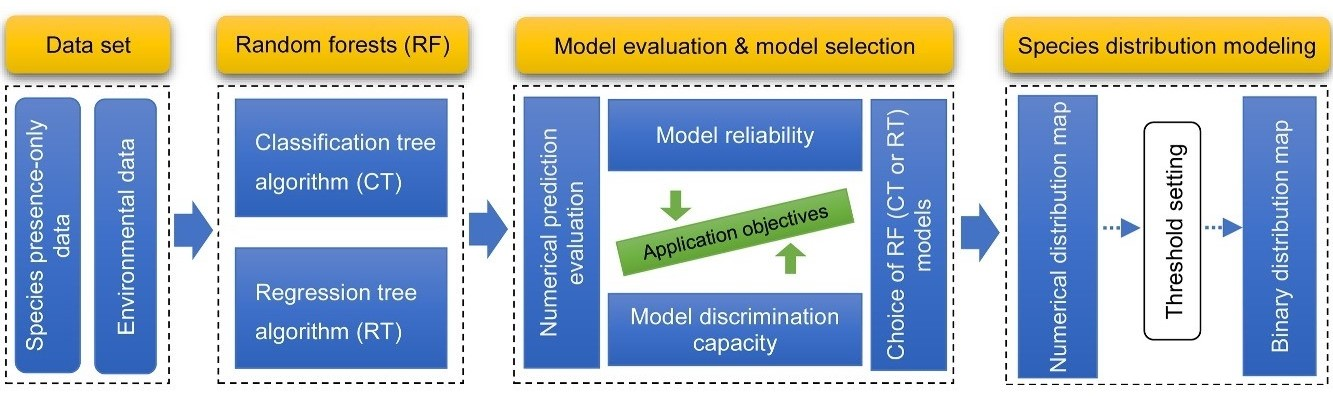
\includegraphics[width = \textwidth]{Workflow.jpg}
        \caption{The use of classification and regression algorithms using the random forests method with presence-only data to model species distribution, Zhang, Huettmann, et.al }
    \end{figure}
    \end{center}
\end{frame}





\begin{frame}{Species Distribution Models}
    \begin{itemize}
        \item RandomForest and TreeNet(Boosted Trees) Models were fitted using Salford Predictive Modeler. 
        \begin{center}
            
\includegraphics[width = .5\textwidth]{SPM image.png}
        \end{center}
        \vfill
        \item RandomForest
        \begin{itemize}
            \item 500 trees.
            \item Minimum of 2 samples per leaf. 
            \item Bootstrapped 3 predictors and 94,000 observations(WR).
        \end{itemize}
        \vfill
        \item TreeNet
        \begin{itemize}
            \item 500 trees. 
            \item Maximum of 6 nodes per tree.
            \item Bootstrapped 3 predictors and 94,000 observations(WR).
        \end{itemize}
    \end{itemize}
\end{frame}





\begin{frame}{Results}
    \begin{figure}
    \begin{center}
    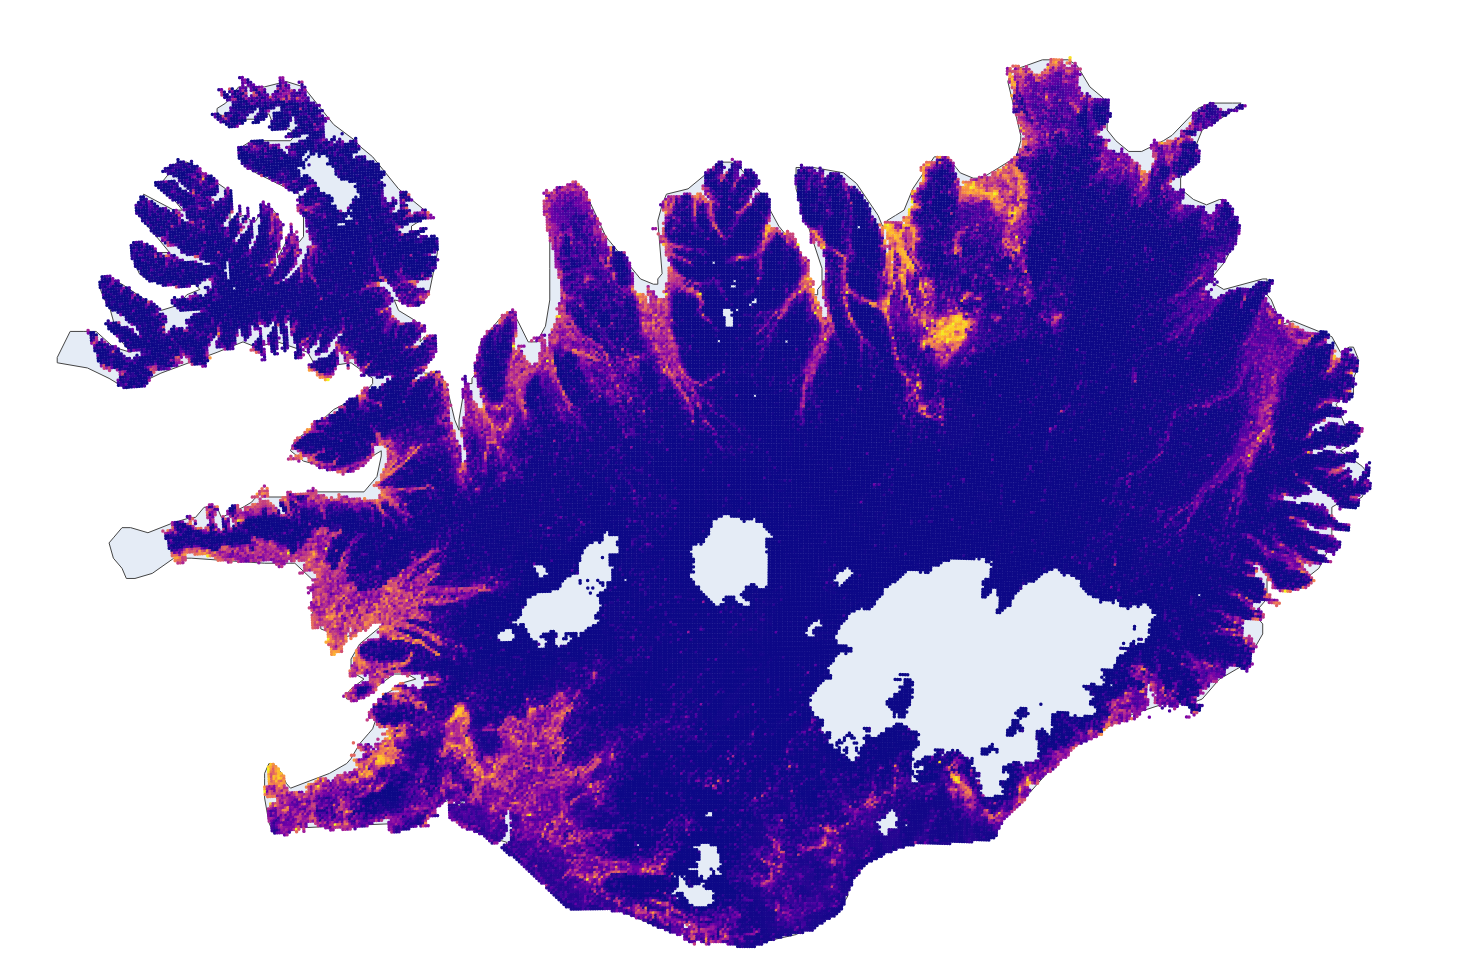
\includegraphics[width = .9\textwidth]{figRFMrio.png}
    \caption{Random Forest Model}
\end{center}
\end{figure}
\end{frame}


\begin{frame}{Results}
    \begin{figure}
    \begin{center}
    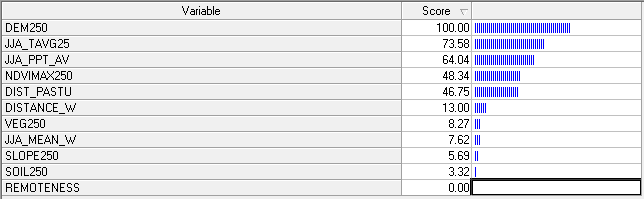
\includegraphics[width = .9\textwidth]{RandomForestVariableImportance.png}
    \caption{Random Forest Variable Importance}
\end{center}
\end{figure}
\end{frame}


\begin{frame}{Results}
\begin{columns}[T]
    \begin{column}{.35 \textwidth}
        \begin{itemize}
            \item Accuracy of $91.98\%$ on out of bag samples. 
        \end{itemize}
    \end{column}
    
    \begin{column}{.65\textwidth}
    \begin{center}
        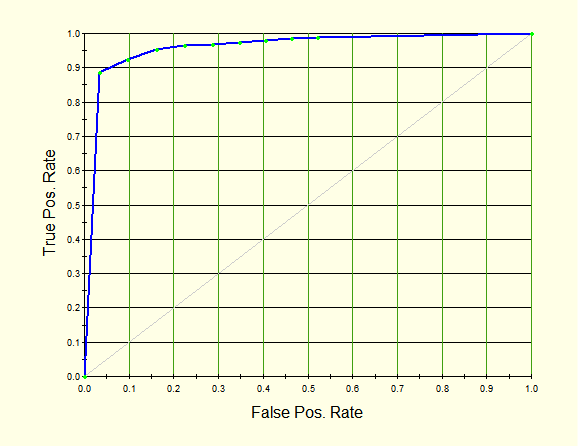
\includegraphics[width = \textwidth]{ROCcurveOOB.png}
    \end{center}
    \end{column}
\end{columns}
\end{frame}

\begin{frame}{Results}
    \begin{columns}[T]
        \begin{column}{.35 \textwidth}
            \begin{itemize}
                \item Accuracy of $72.91\%$ on outside data with kriged predictors.
            \end{itemize}   
        \end{column}
        
        \begin{column}{.65\textwidth}
        \begin{center}
            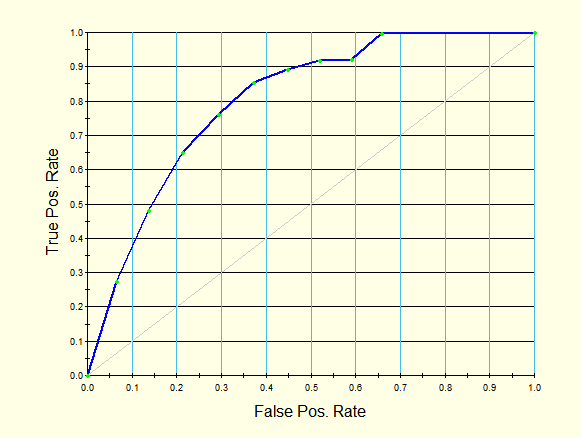
\includegraphics[width = \textwidth]{ROCcurveKriged.png}
        \end{center}
        \end{column}
    \end{columns}
    \end{frame}





    \begin{frame}{Results}
        \begin{figure}
        \begin{center}
        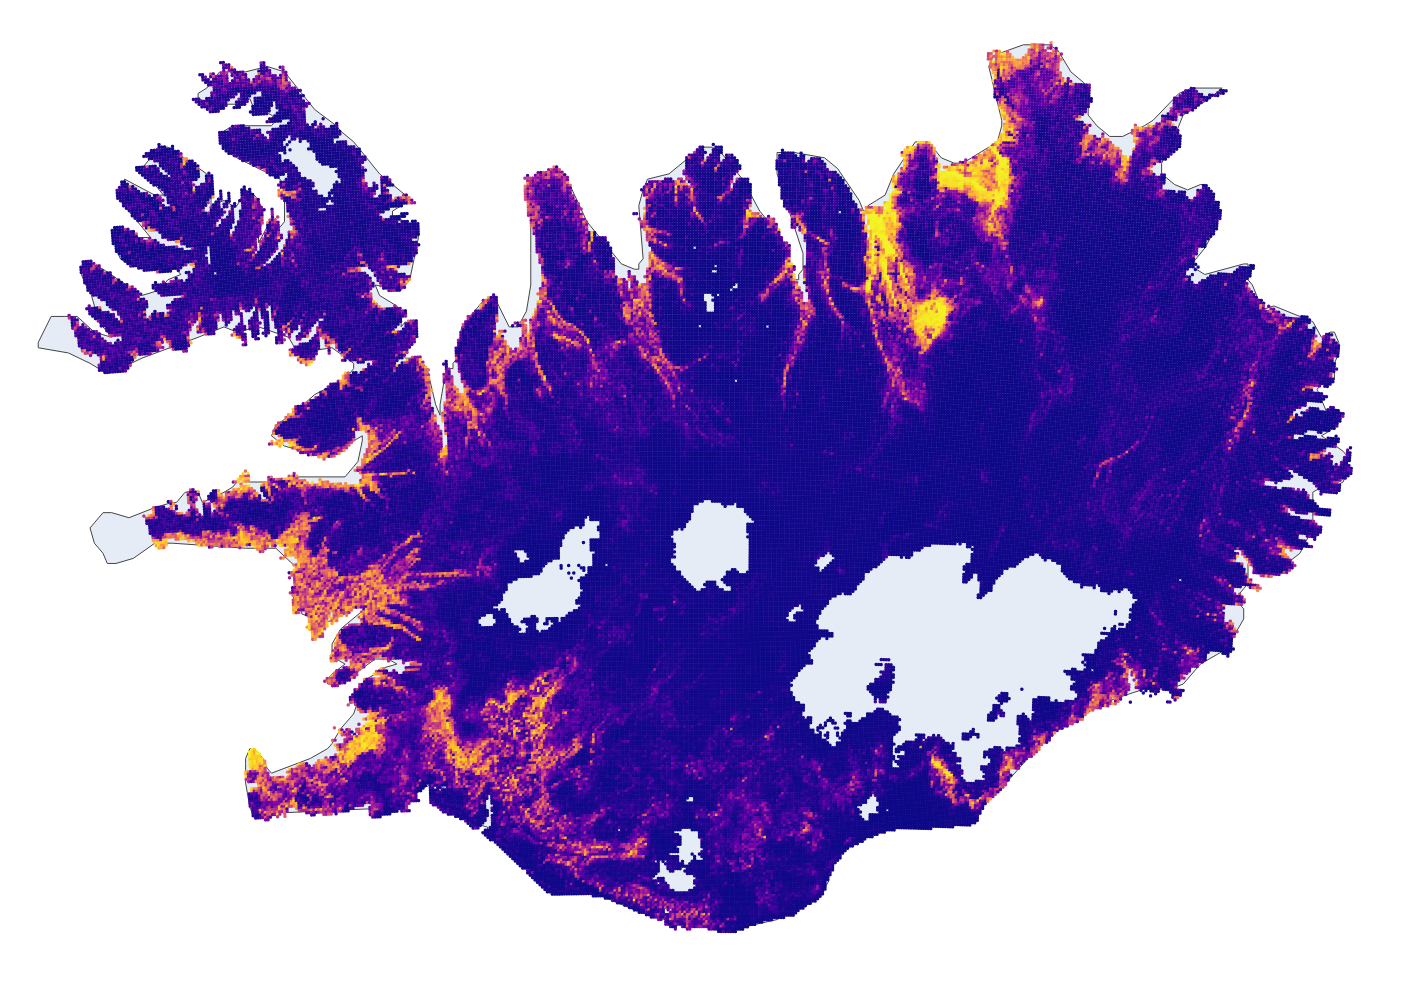
\includegraphics[width = .9\textwidth]{figGBMrio.png}
        \caption{TreeNet(Boosted Tree) Model}
    \end{center}
    \end{figure}
    \end{frame}
    


    \begin{frame}{Results}
        \begin{figure}
        \begin{center}
        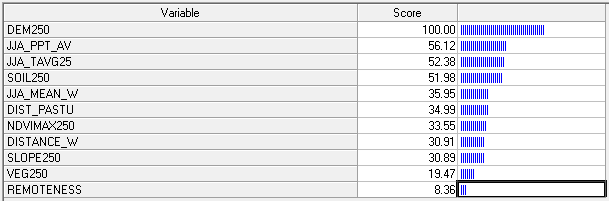
\includegraphics[width = .9\textwidth]{GradiantBoostVariableImportance.png}
        \caption{TreeNet(Boosted Tree) Variable Importance}
    \end{center}
    \end{figure}
    \end{frame}
    
    
    \begin{frame}{Results}
    \begin{columns}[T]
        \begin{column}{.35 \textwidth}
            \begin{itemize}
                \item Accuracy of $91.77\%$ on Cross-Validated samples. 
            \end{itemize}
        \end{column}
        
        \begin{column}{.65\textwidth}
        \begin{center}
            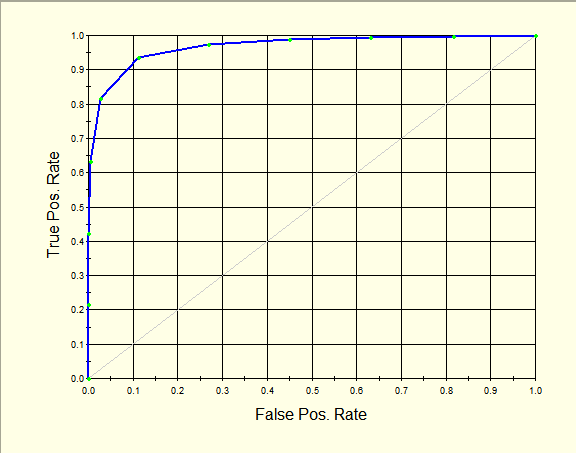
\includegraphics[width = \textwidth]{ROCGBMCV.png}
        \end{center}
        \end{column}
    \end{columns}
    \end{frame}
    
    \begin{frame}{Results}
        \begin{columns}[T]
            \begin{column}{.35 \textwidth}
                \begin{itemize}
                    \item Accuracy of $80.78\%$ on outside data with kriged predictors.
                \end{itemize}   
            \end{column}
            
            \begin{column}{.65\textwidth}
            \begin{center}
                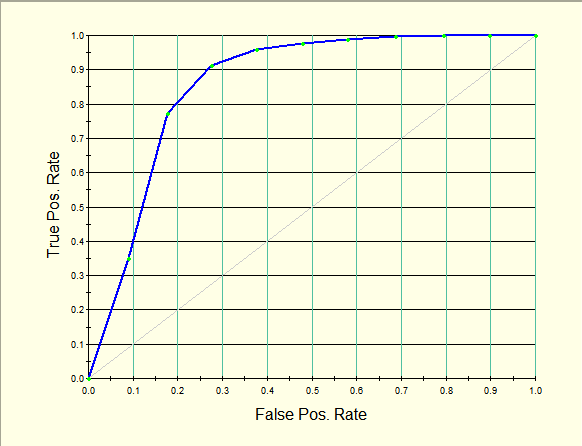
\includegraphics[width = \textwidth]{ROCGBMKriged.png}
            \end{center}
            \end{column}
        \end{columns}
        \end{frame}


        \begin{frame}{Learnings}
            \begin{itemize}
                \item In all models Elevation, Precipitation, and Temperature were the most significant predictors. 
                \item Issues with model training, specifically bootstrapping and spatial autocorrelation, 
                \begin{figure}
                    \begin{center}
                    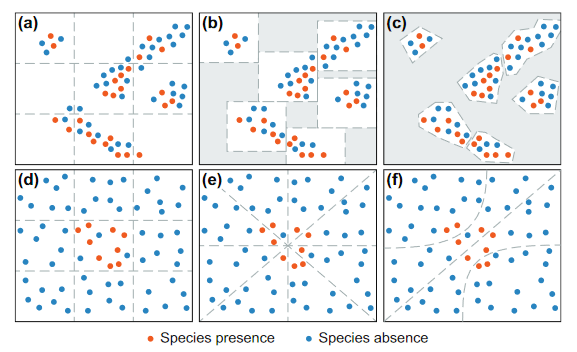
\includegraphics[width = .7\textwidth]{ExamplesOfBlockValidation.png}
                    \caption{Cross-validation strategies for data with temporal, spatial, hierarchical, or phylogenetic structure... Roberts et.al}
                \end{center}
                \end{figure}
            \end{itemize}
            
        \end{frame}

\end{document}






## Outline



 - What is Multivariable Spatial Prediction 
     - Building up from kriging, co-kriging we add auxilliary varaibles(covariates), MSP allows covariates and multiple maps or layers. 
     - Technical definition 
     - Examples of Applications in Ecology/GeoSciences. 


- My Project and Data Specifically
     My Project involves mapping the habitability of the rock ptarmgin species accross all of iceland. 
     We used several of these enviornmental layers to create a Relative Index of occourance or habitablity score using
     by predicting presence absence using these enviornmental layers and several decision tree models. 


Introduction: The Goal
 - Applications in Ecology/GeoSciences
Expand the kriging maps into a multivariate dimentsion. 
Many times in ecology/wildlife/Geoscience we are using the massive enviornmental 
layers, regularly spaced data taken from satellites like elevation, land cover, vegitation
or Soil quality. THese things all closely intereact so it would be nice to be able to incorporate 
their connection to enhance our prediction of these layers. 


 - Recall the general outline of regular Kriging

 - Explain the expansion into coKriging

 - Code

 - Application to our data set 

 - results from model validation. 



 land cover classes, soil types, wilderness; and eight
  continuous variables: elevation, Euclidean distance to fenced pastures, 
  Euclidean distance to water (inland), Normalized Difference Vegetation Index (NDVI), 
  slope, as well as average precipitation, temperature and wind speed for June, July and August.


  Predictor variable raster files were tested for multicollinearity 
  using the cor function in the caret package (Kuhn, 2021); none showed a correlation above 0.75.


  Lambert 2016 Icelandic Projection.


  http://fisher.stats.uwo.ca/faculty/kulperger/S9934a/Papers/Pebesma2004.pdf
  https://link.springer.com/content/pdf/10.1007/BF00893273.pdf
  https://upcommons.upc.edu/bitstream/handle/2117/116322/Giraldo,+Delicado+&+Mateu.+2017.+Cokriging+and+multivariate+kriging+methods+based+on+data+of+a+functional+random+field.pdf;jsessionid=0CF25A137AF10296A24C5CD866ACB8BC?sequence=1

  https://petrowiki.spe.org/Kriging_and_cokriging#Cokriging_estimator
